% =====================================================================
%  Research-paper version. Compile: latexmk -pdf paper.tex  (or upload the folder to Overleaf)
%  Every number comes from generated/*.tex (python -m irp.collect). Body text can be moved into
%  any venue template (IEEEtran etc.) without changes: only sections, tables, figures and macros are used.
% =====================================================================
\documentclass[10pt,twocolumn,a4paper]{article}

\usepackage[a4paper,margin=1.7cm,columnsep=0.6cm]{geometry}
\usepackage[T1]{fontenc}
\usepackage{mathptmx}
\usepackage{microtype}
\usepackage{graphicx}
\usepackage{booktabs}
\usepackage{array}
\usepackage{amsmath,amssymb}
\usepackage{caption}
\usepackage{xcolor}
\usepackage{enumitem}
\usepackage[hidelinks]{hyperref}

% Auto-generated by irp.collect - do not edit.
\providecommand{\mDuration}{}\renewcommand{\mDuration}{24.1}
\providecommand{\mFramesAnalysed}{}\renewcommand{\mFramesAnalysed}{694}
\providecommand{\mTracks}{}\renewcommand{\mTracks}{39}
\providecommand{\mPolice}{}\renewcommand{\mPolice}{8}
\providecommand{\mDirRL}{}\renewcommand{\mDirRL}{20}
\providecommand{\mDirLR}{}\renewcommand{\mDirLR}{11}
\providecommand{\mDirTo}{}\renewcommand{\mDirTo}{5}
\providecommand{\mDirAway}{}\renewcommand{\mDirAway}{3}
\providecommand{\mOccMean}{}\renewcommand{\mOccMean}{9.6}
\providecommand{\mOccPNN}{}\renewcommand{\mOccPNN}{20.5}
\providecommand{\mOccPeak}{}\renewcommand{\mOccPeak}{26.9}
\providecommand{\mOccPeakT}{}\renewcommand{\mOccPeakT}{21.8}
\providecommand{\mVest}{}\renewcommand{\mVest}{98.6}
\providecommand{\mSpeed}{}\renewcommand{\mSpeed}{1.72}
\providecommand{\mRoadArea}{}\renewcommand{\mRoadArea}{49.1}
\providecommand{\mZebra}{}\renewcommand{\mZebra}{11}
\providecommand{\mTrackDur}{}\renewcommand{\mTrackDur}{1.6}
\providecommand{\mMeanUsers}{}\renewcommand{\mMeanUsers}{3.45}
\providecommand{\mWall}{}\renewcommand{\mWall}{40.3}
\providecommand{\mProcFps}{}\renewcommand{\mProcFps}{18.0}
\providecommand{\mOpenCV}{}\renewcommand{\mOpenCV}{5.0.0}
\providecommand{\mNumpy}{}\renewcommand{\mNumpy}{2.5.4}
\providecommand{\mNSOccMean}{}\renewcommand{\mNSOccMean}{13.0}
\providecommand{\mNSOccPNN}{}\renewcommand{\mNSOccPNN}{28.0}
\providecommand{\mNSOccPeak}{}\renewcommand{\mNSOccPeak}{33.6}
\providecommand{\mNSTracks}{}\renewcommand{\mNSTracks}{42}
\providecommand{\mNSPolice}{}\renewcommand{\mNSPolice}{9}
\providecommand{\mShadowGainPP}{}\renewcommand{\mShadowGainPP}{3.5}
\providecommand{\mShadowGainRel}{}\renewcommand{\mShadowGainRel}{36}
\providecommand{\mMtLowTracks}{}\renewcommand{\mMtLowTracks}{43}
\providecommand{\mMtLowL}{}\renewcommand{\mMtLowL}{8}
\providecommand{\mMtHighTracks}{}\renewcommand{\mMtHighTracks}{28}
\providecommand{\mMtHighL}{}\renewcommand{\mMtHighL}{20}
\providecommand{\mFiveDur}{}\renewcommand{\mFiveDur}{5.0}
\providecommand{\mFiveTracks}{}\renewcommand{\mFiveTracks}{11}
\providecommand{\mFiveOccMean}{}\renewcommand{\mFiveOccMean}{5.7}
\providecommand{\mFiveOccPeak}{}\renewcommand{\mFiveOccPeak}{10.4}
\providecommand{\mFiveVest}{}\renewcommand{\mFiveVest}{100.0}
\providecommand{\mTests}{}\renewcommand{\mTests}{56}
\providecommand{\mTestsStatus}{}\renewcommand{\mTestsStatus}{all passed}

% Auto-generated by irp.collect (paper macros) - do not edit.
\providecommand{\mBDuration}{}\renewcommand{\mBDuration}{118.8}
\providecommand{\mBFrames}{}\renewcommand{\mBFrames}{3534}
\providecommand{\mBTracks}{}\renewcommand{\mBTracks}{215}
\providecommand{\mBPolice}{}\renewcommand{\mBPolice}{3}
\providecommand{\mBDirRL}{}\renewcommand{\mBDirRL}{143}
\providecommand{\mBDirLR}{}\renewcommand{\mBDirLR}{65}
\providecommand{\mBDirTo}{}\renewcommand{\mBDirTo}{6}
\providecommand{\mBDirAway}{}\renewcommand{\mBDirAway}{1}
\providecommand{\mBOccMean}{}\renewcommand{\mBOccMean}{4.4}
\providecommand{\mBOccPNN}{}\renewcommand{\mBOccPNN}{14.0}
\providecommand{\mBOccPeak}{}\renewcommand{\mBOccPeak}{35.5}
\providecommand{\mBOccPeakT}{}\renewcommand{\mBOccPeakT}{16.7}
\providecommand{\mBSpeed}{}\renewcommand{\mBSpeed}{2.35}
\providecommand{\mBTrackDur}{}\renewcommand{\mBTrackDur}{1.6}
\providecommand{\mBVest}{}\renewcommand{\mBVest}{0.9}
\providecommand{\mBFps}{}\renewcommand{\mBFps}{115.3}
\providecommand{\mBMeanUsers}{}\renewcommand{\mBMeanUsers}{2.53}
\providecommand{\mBRoadArea}{}\renewcommand{\mBRoadArea}{52.2}
\providecommand{\mBCrossVRL}{}\renewcommand{\mBCrossVRL}{89}
\providecommand{\mBCrossVLR}{}\renewcommand{\mBCrossVLR}{8}
\providecommand{\mBCrossHToward}{}\renewcommand{\mBCrossHToward}{40}
\providecommand{\mBCrossHAway}{}\renewcommand{\mBCrossHAway}{15}
\providecommand{\mBHeadMed}{}\renewcommand{\mBHeadMed}{0.44}
\providecommand{\mBHeadMean}{}\renewcommand{\mBHeadMean}{1.16}
\providecommand{\mBBurstN}{}\renewcommand{\mBBurstN}{4}
\providecommand{\mBBurstDur}{}\renewcommand{\mBBurstDur}{14.1}
\providecommand{\mBBurstInt}{}\renewcommand{\mBBurstInt}{33.8}
\providecommand{\mBBurstCV}{}\renewcommand{\mBBurstCV}{0.51}
\providecommand{\mBGreedyTracks}{}\renewcommand{\mBGreedyTracks}{166}
\providecommand{\mBGreedyOcc}{}\renewcommand{\mBGreedyOcc}{4.4}
\providecommand{\mBEnhTracks}{}\renewcommand{\mBEnhTracks}{253}
\providecommand{\mBEnhOcc}{}\renewcommand{\mBEnhOcc}{5.1}
\providecommand{\mBEnhR}{}\renewcommand{\mBEnhR}{0.966}
\providecommand{\mBEnhMae}{}\renewcommand{\mBEnhMae}{0.84}
\providecommand{\mBNSTracks}{}\renewcommand{\mBNSTracks}{227}
\providecommand{\mBNSOcc}{}\renewcommand{\mBNSOcc}{5.9}
\providecommand{\mBNSGain}{}\renewcommand{\mBNSGain}{1.5}
\providecommand{\mBNSGainRel}{}\renewcommand{\mBNSGainRel}{35}
\providecommand{\mRobMinR}{}\renewcommand{\mRobMinR}{0.963}
\providecommand{\mRobMinRNone}{}\renewcommand{\mRobMinRNone}{0.964}
\providecommand{\mRobMaxR}{}\renewcommand{\mRobMaxR}{0.998}
\providecommand{\mRobMaxTrackDev}{}\renewcommand{\mRobMaxTrackDev}{37}
\providecommand{\mRobMeanR}{}\renewcommand{\mRobMeanR}{0.985}
\providecommand{\mRobMeanRFull}{}\renewcommand{\mRobMeanRFull}{0.982}
\providecommand{\mRobNConds}{}\renewcommand{\mRobNConds}{8}
\providecommand{\mRobMaeNone}{}\renewcommand{\mRobMaeNone}{1.48}
\providecommand{\mRobMaeFull}{}\renewcommand{\mRobMaeFull}{1.49}
\providecommand{\mRobEnhBetter}{}\renewcommand{\mRobEnhBetter}{5}
\providecommand{\mRobComboRN}{}\renewcommand{\mRobComboRN}{0.964}
\providecommand{\mRobComboMaeN}{}\renewcommand{\mRobComboMaeN}{1.71}
\providecommand{\mRobComboRF}{}\renewcommand{\mRobComboRF}{0.963}
\providecommand{\mRobComboMaeF}{}\renewcommand{\mRobComboMaeF}{1.41}
\providecommand{\mRobResLowRN}{}\renewcommand{\mRobResLowRN}{0.982}
\providecommand{\mRobResLowMaeN}{}\renewcommand{\mRobResLowMaeN}{3.16}
\providecommand{\mRobResLowRF}{}\renewcommand{\mRobResLowRF}{0.975}
\providecommand{\mRobResLowMaeF}{}\renewcommand{\mRobResLowMaeF}{4.29}
\providecommand{\mRobCrfRN}{}\renewcommand{\mRobCrfRN}{0.964}
\providecommand{\mRobCrfMaeN}{}\renewcommand{\mRobCrfMaeN}{1.59}
\providecommand{\mRobCrfRF}{}\renewcommand{\mRobCrfRF}{0.964}
\providecommand{\mRobCrfMaeF}{}\renewcommand{\mRobCrfMaeF}{1.55}
\providecommand{\mRobRefTracks}{}\renewcommand{\mRobRefTracks}{46}
\providecommand{\mRobRefOcc}{}\renewcommand{\mRobRefOcc}{9.56}
\providecommand{\mBenchGCleanFrag}{}\renewcommand{\mBenchGCleanFrag}{1.55}
\providecommand{\mBenchGCleanIdsw}{}\renewcommand{\mBenchGCleanIdsw}{6}
\providecommand{\mBenchGCleanPur}{}\renewcommand{\mBenchGCleanPur}{0.881}
\providecommand{\mBenchKCleanFrag}{}\renewcommand{\mBenchKCleanFrag}{1.0}
\providecommand{\mBenchKCleanIdsw}{}\renewcommand{\mBenchKCleanIdsw}{0}
\providecommand{\mBenchKCleanPur}{}\renewcommand{\mBenchKCleanPur}{0.998}
\providecommand{\mBenchGMissedFrag}{}\renewcommand{\mBenchGMissedFrag}{3.294}
\providecommand{\mBenchGMissedIdsw}{}\renewcommand{\mBenchGMissedIdsw}{29}
\providecommand{\mBenchGMissedPur}{}\renewcommand{\mBenchGMissedPur}{0.753}
\providecommand{\mBenchKMissedFrag}{}\renewcommand{\mBenchKMissedFrag}{1.225}
\providecommand{\mBenchKMissedIdsw}{}\renewcommand{\mBenchKMissedIdsw}{2}
\providecommand{\mBenchKMissedPur}{}\renewcommand{\mBenchKMissedPur}{0.983}
\providecommand{\mBenchGOccludedFrag}{}\renewcommand{\mBenchGOccludedFrag}{4.1}
\providecommand{\mBenchGOccludedIdsw}{}\renewcommand{\mBenchGOccludedIdsw}{44}
\providecommand{\mBenchGOccludedPur}{}\renewcommand{\mBenchGOccludedPur}{0.718}
\providecommand{\mBenchKOccludedFrag}{}\renewcommand{\mBenchKOccludedFrag}{1.512}
\providecommand{\mBenchKOccludedIdsw}{}\renewcommand{\mBenchKOccludedIdsw}{6}
\providecommand{\mBenchKOccludedPur}{}\renewcommand{\mBenchKOccludedPur}{0.938}
\providecommand{\mBenchGDenseFrag}{}\renewcommand{\mBenchGDenseFrag}{7.633}
\providecommand{\mBenchGDenseIdsw}{}\renewcommand{\mBenchGDenseIdsw}{222}
\providecommand{\mBenchGDensePur}{}\renewcommand{\mBenchGDensePur}{0.53}
\providecommand{\mBenchKDenseFrag}{}\renewcommand{\mBenchKDenseFrag}{2.12}
\providecommand{\mBenchKDenseIdsw}{}\renewcommand{\mBenchKDenseIdsw}{30}
\providecommand{\mBenchKDensePur}{}\renewcommand{\mBenchKDensePur}{0.881}
\providecommand{\mBenchSeeds}{}\renewcommand{\mBenchSeeds}{20}
\providecommand{\mQANoise}{}\renewcommand{\mQANoise}{2.10}
\providecommand{\mQABlock}{}\renewcommand{\mQABlock}{1.072}
\providecommand{\mQABpp}{}\renewcommand{\mQABpp}{0.082}
\providecommand{\mQAJitter}{}\renewcommand{\mQAJitter}{0.070}
\providecommand{\mQAOver}{}\renewcommand{\mQAOver}{7.9}
\providecommand{\mQBNoise}{}\renewcommand{\mQBNoise}{3.03}
\providecommand{\mQBBlock}{}\renewcommand{\mQBBlock}{1.069}
\providecommand{\mQBBpp}{}\renewcommand{\mQBBpp}{0.077}
\providecommand{\mQBJitter}{}\renewcommand{\mQBJitter}{0.017}
\providecommand{\mQBOver}{}\renewcommand{\mQBOver}{11.0}


\captionsetup{font=small,labelfont=bf}
\setlength{\parskip}{0.2em}
\setlist{itemsep=1pt,topsep=2pt,leftmargin=1.2em}
\graphicspath{{figures/}}
\newcommand{\pct}[1]{#1\,\%}

\title{\vspace{-0.6cm}\textbf{Quality-Aware Perception of Unstructured Indian Junction Traffic\\ from Low-Quality Fixed-Camera Video}}
\author{Vishwas N\\ \small M.Tech, Department of DECE, M.\,S.\ Ramaiah Institute of Technology, Bengaluru}
\date{}

\begin{document}
\twocolumn[
\maketitle
\begin{abstract}
\noindent
Low-cost fixed cameras at Indian junctions produce low-resolution, compressed video of dense, lane-free traffic under harsh sunlight.
We study how far classical vision, with no trained models and no labels, can go on such footage, and we separate what is measured from what is assumed.
We present (i) a resolution-adaptive pipeline with shadow-suppressed motion segmentation, a video-quality profile, optional enhancement and stabilisation;
(ii) a Kalman + Hungarian tracker, checked on simulated traffic with exact ground truth, where it cuts identity switches from \mBenchGDenseIdsw\ to \mBenchKDenseIdsw\ per sequence in dense traffic;
(iii) a reference-based degradation study of \mRobNConds\ conditions (resolution, blur, noise, H.264 compression, and a combined condition) in which
road-occupancy time series keep a Pearson correlation of at least \mRobMinR\ with the high-quality reference in every condition;
and (iv) flow analytics (counting gates, headways, traffic bursts) with a persistence rule that rejects orange vehicles as police vests.
On a \mBDuration\,s, $640\times360$ junction clip the pipeline tracks \mBTracks\ road users, counts \mBCrossVRL\ right-to-left crossings of a mid-image gate, and finds \mBBurstN\ traffic bursts.
Enhancement is not uniformly beneficial: it lowers the mean occupancy error in \mRobEnhBetter\ of \mRobNConds\ degradation conditions but not on average (\mRobMaeNone\ versus \mRobMaeFull\,pp).
Code, tests and all results are reproducible with one command; no human-labelled ground truth exists for the real clips, and we state the consequences.
\end{abstract}
\vspace{0.3cm}
]

% =====================================================================
\section{Introduction}
% =====================================================================
Indian junctions combine heterogeneous traffic (two-wheelers, auto-rickshaws, cars, buses, pedestrians), weak lane discipline and manual traffic control.
Detectors and segmenters trained on structured datasets degrade in such scenes, and fine-tuning on India Driving Dataset (IDD)~\cite{varma2019} is the long-term route.
Before and alongside that, inexpensive scene-level measurements (flow, occupancy, bursts) from existing low-quality cameras are already useful, provided their reliability under poor video quality is known.
This paper asks three questions: \emph{(Q1)} how does video quality affect classical scene measurements; \emph{(Q2)} which tracker design is justified when ground truth is unavailable; \emph{(Q3)} what can be inferred from a real 360p junction clip?

\textbf{Contributions.} (1) A quality-profiling, resolution-adaptive static-camera pipeline with shadow suppression, optional enhancement and stabilisation.
(2) A Kalman + Hungarian tracker and a controlled benchmark with exact ground truth.
(3) A reference-based degradation protocol that needs no labels.
(4) Flow analytics, including headways, traffic bursts and a persistence rule for the traffic-police cue.
(5) An open, tested, one-command reproducible code base.

% =====================================================================
\section{Related Work}
% =====================================================================
\textbf{Detection and segmentation.} YOLO-family detectors~\cite{redmon2016} and SegFormer~\cite{xie2021} are the standard deep-learning route; IDD~\cite{varma2019} provides unstructured-road labels.
\textbf{Background subtraction.} Gaussian-mixture models~\cite{stauffer1999,zivkovic2004} are cheap and training-free; shadows are a known failure source~\cite{prati2003}.
\textbf{Tracking.} Tracking by detection with Kalman filtering and Hungarian assignment~\cite{kalman1960,kuhn1955,bewley2016} and ByteTrack~\cite{zhang2022} are widely used; tracking quality is conventionally scored with CLEAR-MOT metrics~\cite{bernardin2008}.
\textbf{Video quality.} Noise estimation~\cite{immerkaer1996}, local contrast enhancement~\cite{zuiderveld1994}, bilateral filtering~\cite{tomasi1998} and phase correlation~\cite{kuglin1975} are the classical building blocks used here.

% =====================================================================
\section{Method}
% =====================================================================
\subsection{Quality profile}
For each clip we report resolution, bits per pixel of the file, noise $\sigma$ (Immerkaer estimator~\cite{immerkaer1996}), blockiness (mean gradient on 8-pixel block boundaries divided by elsewhere), Laplacian-variance sharpness at a common width, over-exposed pixel fraction, and inter-frame jitter from phase correlation of the static upper image region.
Flags use rule-of-thumb thresholds and are not validated standards; sharpness depends on scene content and is compared only within a scene.

\subsection{Resolution-adaptive motion segmentation}
A temporal median of 60 frames gives the background and the road mask (low saturation, below the far road edge, largest component).
Motion is segmented with MOG2~\cite{zivkovic2004}: each pixel is a Gaussian mixture $p(\mathbf{x}_t)=\sum_k\pi_k\mathcal{N}(\mathbf{x}_t;\boldsymbol\mu_k,\sigma_k^2\mathbf{I})$, and pixels labelled as shadow are discarded.
All pixel parameters are defined at 960\,px width and scaled by $s=W_p/960$ (kernels, minimum blob size, tracking radius, displacement threshold), so identical settings run from 320 to 960\,px.
Road occupancy is $O_t=|F_t\cap\mathcal{D}(R)|/|R|$ for foreground $F_t$, road $R$ and dilation $\mathcal{D}$.
Optional enhancement applies a light bilateral filter and CLAHE~\cite{zuiderveld1994,tomasi1998} on luminance; optional stabilisation removes accumulated translation estimated on the static upper region.

\subsection{Tracking}
Each track carries a constant-velocity Kalman state $\mathbf{x}=[x,y,\dot x,\dot y]^{\top}$ with $\mathbf{x}_{t|t-1}=\mathbf{F}\mathbf{x}_{t-1}$ and measurement update $\mathbf{x}_t=\mathbf{x}_{t|t-1}+\mathbf{K}(\mathbf{z}_t-\mathbf{H}\mathbf{x}_{t|t-1})$.
Detections are assigned to predicted tracks by the Hungarian algorithm with cost $0.5\,d/d_{\max}+0.5\,(1-\mathrm{IoU})$ and a distance gate $d\le d_{\max}$; unmatched tracks coast on their prediction for up to 10 frames.
The baseline is greedy nearest-centroid matching.

\subsection{Flow analytics and traffic bursts}
A \emph{gate} is a segment in normalised image coordinates; a track whose base point crosses it is counted with its direction (a point exactly on the line counts as the negative side so that no crossing is lost).
Headways are gaps between consecutive crossings of a gate. A \emph{burst} is a period where the 1\,s smoothed occupancy exceeds $0.35$ times its 95th percentile (minimum 0.01), merged across gaps shorter than 3\,s and kept if longer than 2\,s.
On signalised junctions bursts may follow the signal cycle; this is a hypothesis, not an assumption.

\subsection{Traffic-police cue}
Orange hi-vis blobs (HSV thresholds, size and aspect limits) are accepted as police only if blobs recur around the same place for at least 2\,s (a 3$\times$3 grid-cell neighbourhood), because on-duty personnel stand still while orange vehicles move; tracks containing an accepted vest are excluded from traffic statistics.

% =====================================================================
\section{Experimental Protocol}
% =====================================================================
\textbf{Data.} Clip~A: $1280\times720$, 24.1\,s, junction with two traffic police. Clip~B: $640\times360$, \mBDuration\,s, a different junction with intermittent traffic.
Both are fixed-camera recordings; no human labels exist.

\textbf{E1 -- tracker benchmark (exact ground truth).} Simulated crossings with jitter, missed detections, occlusion gaps and false positives (four scenarios, \mBenchSeeds\ seeds each).
Metrics: fragments per object, identity switches, purity, count ratio, false tracks.

\textbf{E2 -- degradation study (reference-based).} Clip~A is degraded with ffmpeg/x264: down-scaling to $640\times360$, $480\times270$, $320\times180$; Gaussian blur ($\sigma=2$); temporal noise (10); CRF 35 and 45; and a combined condition ($640\times360$, noise 6, CRF 40).
Each version is analysed with and without enhancement (Kalman tracker) and compared with the analysis of the original (\mRobRefTracks\ tracks, mean occupancy \mRobRefOcc\,\%):
Pearson $r$ of the occupancy series, mean absolute occupancy difference in percentage points (MAE), ratio of mean occupancies and of track counts.

\textbf{E3 -- case study on clip B.} Quality profile, tracker, enhancement and shadow ablations, flow gates and bursts.
\textbf{Reproducibility.} \texttt{make all} runs tests, experiments and builds this PDF; all runs are deterministic and their parameters are stored in \texttt{params.json}.

% =====================================================================
\section{Results}
% =====================================================================
\subsection{Video quality}
\begin{table}[t]
\centering
\caption{Quality profile of the two clips (sharpness is scene-dependent).}
\small
\resizebox{\columnwidth}{!}{\begin{tabular}{@{}lrr@{}}
\toprule
Measure & junction1\_720p & junction2\_360p \\
\midrule
Resolution & 1280$\times$720 & 640$\times$360 \\
Duration (s) & 24.1 & 118.8 \\
Bits per pixel (file size) & 0.082 & 0.077 \\
Noise $\sigma$ (grey levels) & 2.10 & 3.03 \\
Blockiness (1 = none) & 1.072 & 1.069 \\
Sharpness (Laplacian variance at 640 px) & 5081 & 2281 \\
Overexposed pixels (\%) & 7.9 & 11.0 \\
Mean brightness / contrast & 120 / 69 & 123 / 75 \\
Inter-frame jitter, RMS (px) & 0.070 & 0.017 \\
Flags & glare\_or\_clipping & low\_resolution, noisy, glare\_or\_clipping \\
\bottomrule
\end{tabular}
}
\label{tab:quality}
\end{table}
Table~\ref{tab:quality} shows that clip~B is low resolution and noisier (noise $\sigma$ \mQBNoise\ versus \mQANoise), with similar compression ($\approx$\mQBBpp\ versus \mQABpp\ bits per pixel) and moderate blockiness (\mQBBlock\ versus \mQABlock).
Both clips have strong glare (\mQBOver\,\% and \mQAOver\,\% over-exposed pixels) and negligible jitter (RMS \mQBJitter\ and \mQAJitter\,px), so stabilisation is not needed for these clips although it is implemented and tested.

\subsection{E1: tracker benchmark}
\begin{table*}[t]
\centering
\caption{Tracker benchmark with exact ground truth (mean$\pm$std over seeds). Ideal: fragments 1, ID switches 0, purity 1, count ratio 1.}
\small
\begin{tabular}{@{}llccccc@{}}
\toprule
Scenario & Tracker & Fragments/object & ID switches & Purity & Count ratio & False tracks \\
\midrule
clean & greedy & 1.55$\pm$0.45 & 5.7$\pm$5.1 & 0.881$\pm$0.102 & 0.96$\pm$0.06 & 0.0$\pm$0.0 \\
 & kalman & 1.00$\pm$0.00 & 0.0$\pm$0.0 & 0.998$\pm$0.009 & 0.99$\pm$0.03 & 0.0$\pm$0.0 \\
missed & greedy & 3.29$\pm$0.59 & 29.0$\pm$10.8 & 0.753$\pm$0.074 & 1.12$\pm$0.10 & 0.0$\pm$0.0 \\
 & kalman & 1.23$\pm$0.27 & 2.2$\pm$2.6 & 0.983$\pm$0.023 & 1.04$\pm$0.09 & 0.0$\pm$0.0 \\
occluded & greedy & 4.10$\pm$0.93 & 44.4$\pm$19.4 & 0.718$\pm$0.081 & 1.24$\pm$0.17 & 0.0$\pm$0.0 \\
 & kalman & 1.51$\pm$0.35 & 6.3$\pm$5.9 & 0.938$\pm$0.053 & 1.11$\pm$0.13 & 0.0$\pm$0.0 \\
dense & greedy & 7.63$\pm$0.74 & 222.1$\pm$35.6 & 0.530$\pm$0.041 & 1.22$\pm$0.10 & 0.0$\pm$0.0 \\
 & kalman & 2.12$\pm$0.41 & 30.4$\pm$11.3 & 0.881$\pm$0.045 & 1.14$\pm$0.10 & 0.0$\pm$0.0 \\
\bottomrule
\end{tabular}

\label{tab:bench}
\end{table*}
The Kalman + Hungarian tracker is better than greedy matching in every scenario (Table~\ref{tab:bench}, Fig.~\ref{fig:bench}).
In the dense scenario it reduces fragments per object from \mBenchGDenseFrag\ to \mBenchKDenseFrag, identity switches from \mBenchGDenseIdsw\ to \mBenchKDenseIdsw, and raises purity from \mBenchGDensePur\ to \mBenchKDensePur.
Even with clean detections greedy matching fragments tracks (\mBenchGCleanFrag\ per object, against \mBenchKCleanFrag\ for Kalman tracking).
These are simulated results; they show that the design is sound, not that real-world counts are correct.

\begin{figure}[t]
\centering
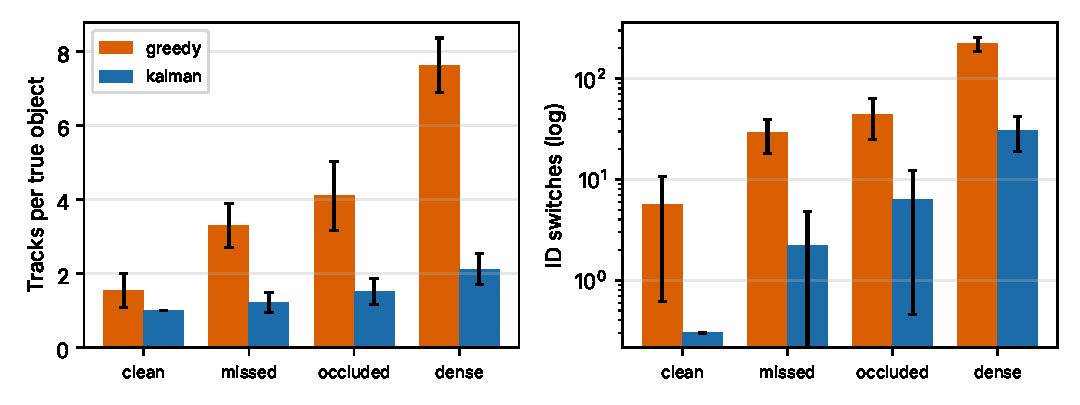
\includegraphics[width=\columnwidth]{fig_benchmark.pdf}
\caption{E1: fragmentation (left) and identity switches (right, log scale) for greedy and Kalman tracking.}
\label{fig:bench}
\end{figure}

\subsection{E2: degradation study}
\begin{table*}[t]
\centering
\caption{E2: agreement of degraded versions of clip~A with the original analysis. $r$: occupancy correlation; MAE: mean absolute occupancy difference (percentage points); ratios are degraded/reference; ``enh.'' = bilateral denoise + CLAHE.}
\small
\begin{tabular}{@{}lcccccccc@{}}
\toprule
 & \multicolumn{2}{c}{Occupancy $r$} & \multicolumn{2}{c}{MAE (pp)} & \multicolumn{2}{c}{Mean ratio} & \multicolumn{2}{c}{Track ratio} \\
Condition & none & enh. & none & enh. & none & enh. & none & enh. \\
\midrule
res360 & 0.994 & 0.990 & 1.59 & 1.05 & 0.83 & 0.89 & 1.28 & 1.13 \\
res270 & 0.987 & 0.983 & 1.92 & 1.43 & 0.80 & 0.85 & 1.04 & 1.22 \\
res180 & 0.982 & 0.975 & 3.16 & 4.29 & 1.33 & 1.45 & 0.78 & 0.83 \\
blur2 & 0.998 & 0.993 & 0.38 & 0.84 & 0.97 & 1.07 & 1.02 & 1.13 \\
noise10 & 0.995 & 0.995 & 1.13 & 0.43 & 0.88 & 0.98 & 0.91 & 1.11 \\
crf35 & 0.997 & 0.991 & 0.32 & 0.96 & 1.00 & 1.09 & 1.22 & 1.06 \\
crf45 & 0.964 & 0.964 & 1.59 & 1.55 & 1.12 & 1.13 & 1.37 & 1.20 \\
combo & 0.964 & 0.963 & 1.71 & 1.41 & 0.86 & 0.91 & 1.13 & 1.24 \\
\bottomrule
\end{tabular}

\label{tab:rob}
\end{table*}
Road occupancy is robust: without enhancement the correlation with the reference stays between \mRobMinRNone\ and \mRobMaxR\ (mean \mRobMeanR) and the mean MAE is \mRobMaeNone\,pp, against a reference mean occupancy of \mRobRefOcc\,\% (Table~\ref{tab:rob}).
Track counts are less robust, deviating from the reference by up to \mRobMaxTrackDev\,\% (Fig.~\ref{fig:rob}).
The effect of enhancement is mixed: it lowers the MAE in \mRobEnhBetter\ of \mRobNConds\ conditions (notably noise and moderate down-scaling) but raises it at $320\times180$ (\mRobResLowMaeN\ to \mRobResLowMaeF\,pp), so that the mean MAE is essentially unchanged (\mRobMaeNone\ versus \mRobMaeFull\,pp).
The combined low-quality condition reaches $r=\mRobComboRN$ (MAE \mRobComboMaeN\,pp) without and $r=\mRobComboRF$ (MAE \mRobComboMaeF\,pp) with enhancement.

\begin{figure}[t]
\centering
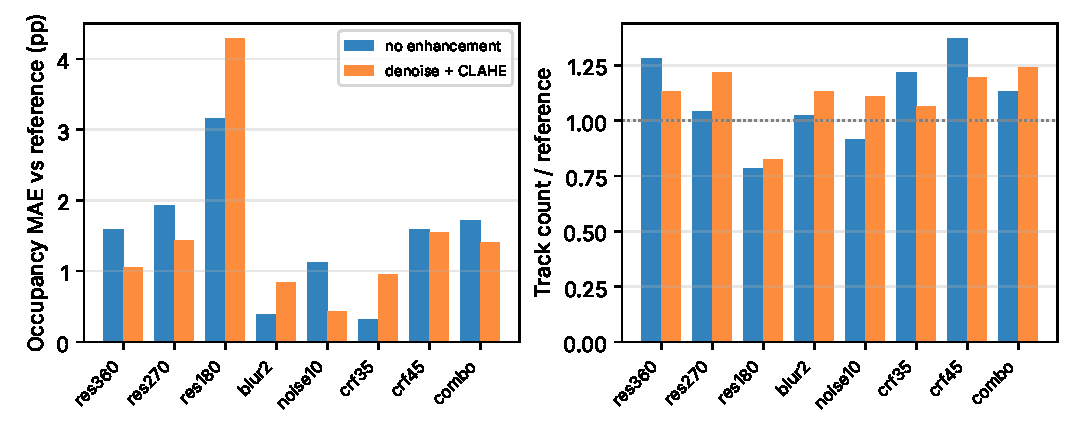
\includegraphics[width=\columnwidth]{fig_robustness.pdf}
\caption{E2: occupancy error (left) and track-count ratio (right) per degradation condition, with and without enhancement.}
\label{fig:rob}
\end{figure}

\subsection{E3: case study on the 360p junction}
\begin{figure*}[t]
\centering
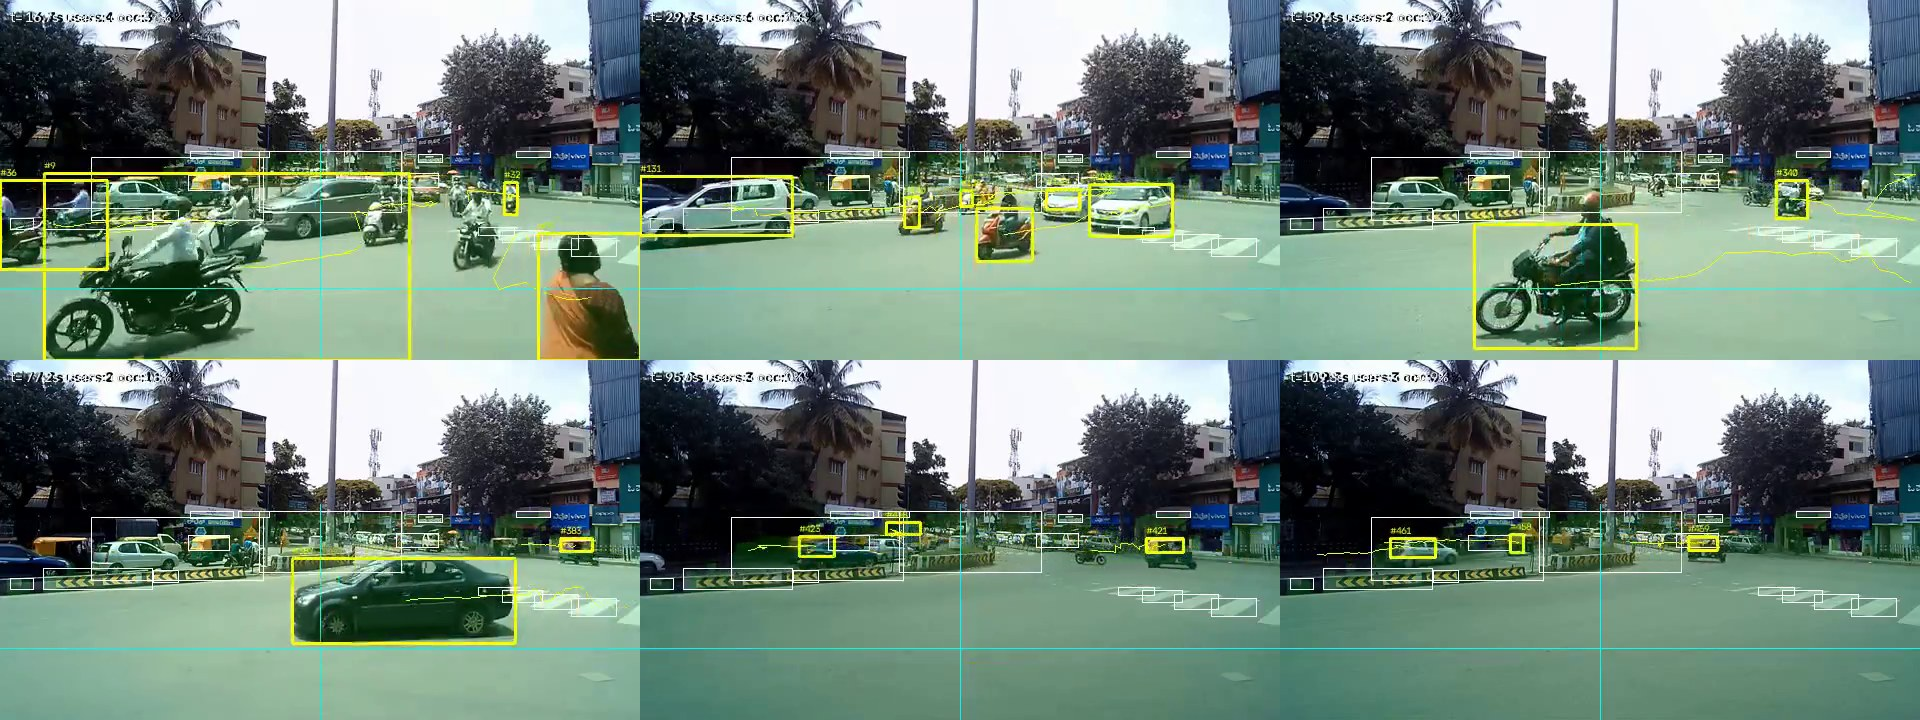
\includegraphics[width=\textwidth]{figB_annotated.jpg}
\caption{Clip~B, annotated frames (road tinted green, gates cyan, tracks yellow with trails). Large boxes can contain several adjacent riders.}
\label{fig:ann}
\end{figure*}
With the Kalman tracker the pipeline tracks \mBTracks\ road users (\mBDirRL\ right-to-left, \mBDirLR\ left-to-right, \mBDirTo\ toward and \mBDirAway\ away from the camera), median relative speed \mBSpeed\ body widths per second, median track duration \mBTrackDur\,s, and mean road occupancy \mBOccMean\,\% (95th percentile \mBOccPNN\,\%, peak \mBOccPeak\,\% at \mBOccPeakT\,s).
The mid-image gate counts \mBCrossVRL\ right-to-left and \mBCrossVLR\ left-to-right crossings; the near gate counts \mBCrossHToward\ toward and \mBCrossHAway\ away from the camera (Table~\ref{tab:flow}); the median headway at the mid gate is \mBHeadMed\,s, so vehicles arrive in groups.
Occupancy shows \mBBurstN\ bursts (mean duration \mBBurstDur\,s, mean start-to-start interval \mBBurstInt\,s, coefficient of variation \mBBurstCV; Fig.~\ref{fig:occB}); with so few bursts, no signal cycle is claimed.
The pipeline ran at \mBFps\ frames per second on a CPU.

\begin{table}[t]
\centering
\caption{E3: gate crossings and headways on clip~B.}
\small
\resizebox{\columnwidth}{!}{\begin{tabular}{@{}lllrrrr@{}}
\toprule
Gate & Direction & Crossings & \multicolumn{4}{c}{Headway, all directions (s)} \\
 & & & n & mean & median & p90 \\
\midrule
mid-vertical &  & L->R: 8, R->L: 89 & 97 & 1.16 & 0.44 & 1.85 \\
near-horizontal &  & away: 15, toward: 40 & 55 & 1.17 & 0.59 & 1.95 \\
\bottomrule
\end{tabular}
}
\label{tab:flow}
\end{table}
\begin{figure}[t]
\centering
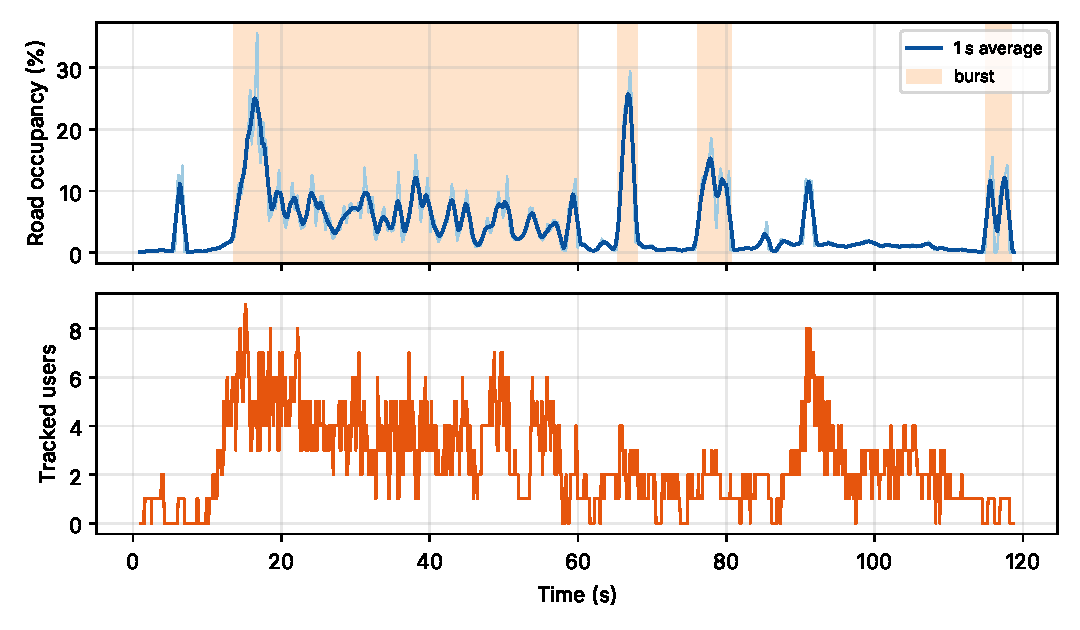
\includegraphics[width=\columnwidth]{figB_occupancy.pdf}
\caption{E3: road occupancy with detected bursts shaded, and tracked users per frame.}
\label{fig:occB}
\end{figure}
\begin{figure}[t]
\centering
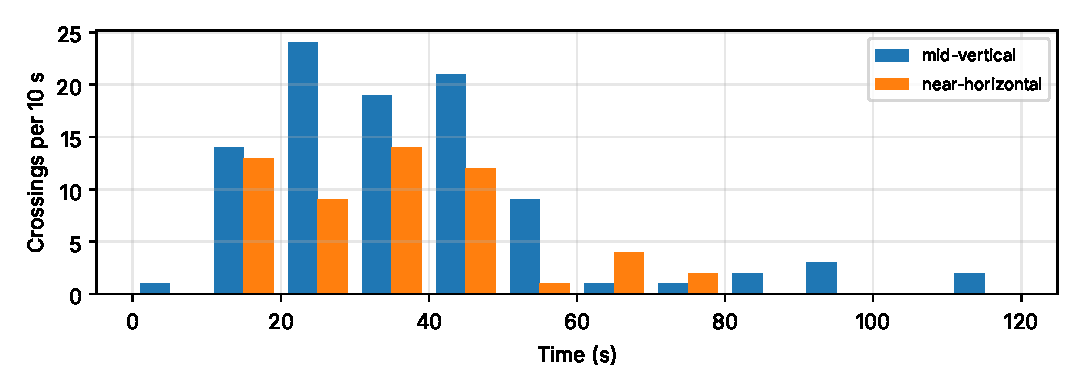
\includegraphics[width=\columnwidth]{figB_flow.pdf}
\caption{E3: gate crossings per 10\,s.}
\label{fig:flowB}
\end{figure}

\textbf{Ablations on clip B.} Counting shadow pixels as foreground raises mean occupancy from \mBOccMean\,\% to \mBNSOcc\,\% (+\mBNSGain\,pp, +\mBNSGainRel\,\% relative), the same direction of error as on clip~A.
Greedy tracking gives \mBGreedyTracks\ tracks against \mBTracks\ for Kalman tracking; enhancement gives \mBEnhTracks\ tracks and a mean occupancy of \mBEnhOcc\,\% (occupancy correlation with the unenhanced run $r=\mBEnhR$, MAE \mBEnhMae\,pp).
Without labels we cannot say which track count is closest to the truth; the benchmark suggests that greedy matching over-fragments identities, but fragmentation can shorten tracks below the confirmation length, so counts need not rise with fragmentation.
The police-vest cue fires in \mBVest\,\% of frames of clip~B, where no police are visible; we did not verify their source, and the persistence rule is a heuristic that also rejects walking officers (an earlier version without it flagged orange vehicles as police in several percent of frames).

% =====================================================================
\section{Discussion and Limitations}
% =====================================================================
\textbf{Findings.} (1) Occupancy is the most robust scene measurement under degradation, counts the least. (2) Shadow suppression matters more than most parameters: ignoring it inflates occupancy by about a third on both clips. (3) Kalman + Hungarian tracking is clearly justified in simulation. (4) Enhancement should be chosen per condition rather than applied by default.

\textbf{Limitations.} No human-labelled ground truth exists for the real clips, so absolute accuracy of counts, directions and bursts is unknown; E2 measures agreement with a reference analysis, not truth, and uses one reference clip; the benchmark is simulated and simpler than real traffic (no merged blobs, constant velocities); several thresholds (burst, vest, quality flags) were set by inspection, not tuned or validated; blob tracking merges adjacent riders into one box; the zebra detector also responds to median markings; the quality flags are heuristic.

\textbf{Future work.} Fine-tune YOLO and SegFormer on IDD and compare with this baseline; annotate a subset of clip~B for CLEAR-MOT and counting error; detector-based tracking to split merged riders; additional junctions to test whether bursts follow signal phases; pose-based recognition of police hand signals.

% =====================================================================
\section{Conclusion}
% =====================================================================
On low-quality fixed-camera video of Indian junctions, classical vision with a quality-aware, resolution-adaptive design yields stable road-occupancy measurements (correlation $\ge$ \mRobMinR\ with a high-quality reference in all conditions), a justified tracker, and useful flow analytics, while counts remain uncertain and enhancement must be judged case by case.
The measurements, tests and code are released as one reproducible package.

\begin{thebibliography}{99}\small
\bibitem{varma2019} G.~Varma \emph{et al.}, ``IDD: A dataset for exploring problems of autonomous navigation in unconstrained environments,'' in \emph{Proc. WACV}, 2019.
\bibitem{redmon2016} J.~Redmon \emph{et al.}, ``You only look once: Unified, real-time object detection,'' in \emph{Proc. CVPR}, 2016.
\bibitem{xie2021} E.~Xie \emph{et al.}, ``SegFormer: Simple and efficient design for semantic segmentation with transformers,'' in \emph{Proc. NeurIPS}, 2021.
\bibitem{stauffer1999} C.~Stauffer and W.~E.~L.~Grimson, ``Adaptive background mixture models for real-time tracking,'' in \emph{Proc. CVPR}, 1999.
\bibitem{zivkovic2004} Z.~Zivkovic, ``Improved adaptive Gaussian mixture model for background subtraction,'' in \emph{Proc. ICPR}, 2004.
\bibitem{prati2003} A.~Prati \emph{et al.}, ``Detecting moving shadows: Algorithms and evaluation,'' \emph{IEEE Trans. PAMI}, vol.~25, no.~7, 2003.
\bibitem{kalman1960} R.~E.~Kalman, ``A new approach to linear filtering and prediction problems,'' \emph{J. Basic Engineering}, vol.~82, no.~1, 1960.
\bibitem{kuhn1955} H.~W.~Kuhn, ``The Hungarian method for the assignment problem,'' \emph{Naval Research Logistics Quarterly}, vol.~2, 1955.
\bibitem{bewley2016} A.~Bewley \emph{et al.}, ``Simple online and realtime tracking,'' in \emph{Proc. ICIP}, 2016.
\bibitem{zhang2022} Y.~Zhang \emph{et al.}, ``ByteTrack: Multi-object tracking by associating every detection box,'' in \emph{Proc. ECCV}, 2022.
\bibitem{bernardin2008} K.~Bernardin and R.~Stiefelhagen, ``Evaluating multiple object tracking performance: The CLEAR MOT metrics,'' \emph{EURASIP J. Image and Video Processing}, 2008.
\bibitem{immerkaer1996} J.~Immerkaer, ``Fast noise variance estimation,'' \emph{Computer Vision and Image Understanding}, vol.~64, no.~2, 1996.
\bibitem{zuiderveld1994} K.~Zuiderveld, ``Contrast limited adaptive histogram equalization,'' in \emph{Graphics Gems IV}, 1994.
\bibitem{tomasi1998} C.~Tomasi and R.~Manduchi, ``Bilateral filtering for gray and color images,'' in \emph{Proc. ICCV}, 1998.
\bibitem{kuglin1975} C.~D.~Kuglin and D.~C.~Hines, ``The phase correlation image alignment method,'' in \emph{Proc. IEEE Int. Conf. Cybernetics and Society}, 1975.
\end{thebibliography}

\end{document}
